\documentclass[tikz,border=5pt]{standalone}

\usetikzlibrary{
  shapes.geometric,
  backgrounds,
  fit,
  arrows.meta,
  positioning,
}

\tikzset{
  task/.style={
    rectangle,
    rounded corners,
    minimum height=2.5em,
    text centered,
    draw=black,
    fill=blue!15
  },
  isr/.style={
    rectangle,
    rounded corners,
    minimum height=2.5em,
    text centered,
    draw=black,
    fill=red!20
  },
  hw_in/.style={
    trapezium,
    trapezium left angle=110,
    trapezium right angle=70,
    minimum height=2em,
    text centered,
    draw=black,
    fill=gray!40
  },
  hw_out/.style={
    trapezium,
    trapezium left angle=70,
    trapezium right angle=110,
    minimum height=2em,
    text centered,
    draw=black,
    fill=gray!40
  },
  callback/.style={
    rectangle,
    dashed,
    minimum height=2.5em,
    text centered,
    draw=black,
    fill=orange!20,
  },
  arrow/.style={
    thick,
    -{Latex[length=3mm]},
  },
  group/.style={
    rectangle,
    rounded corners,
    inner sep=8pt,
  },
}

\begin{document}

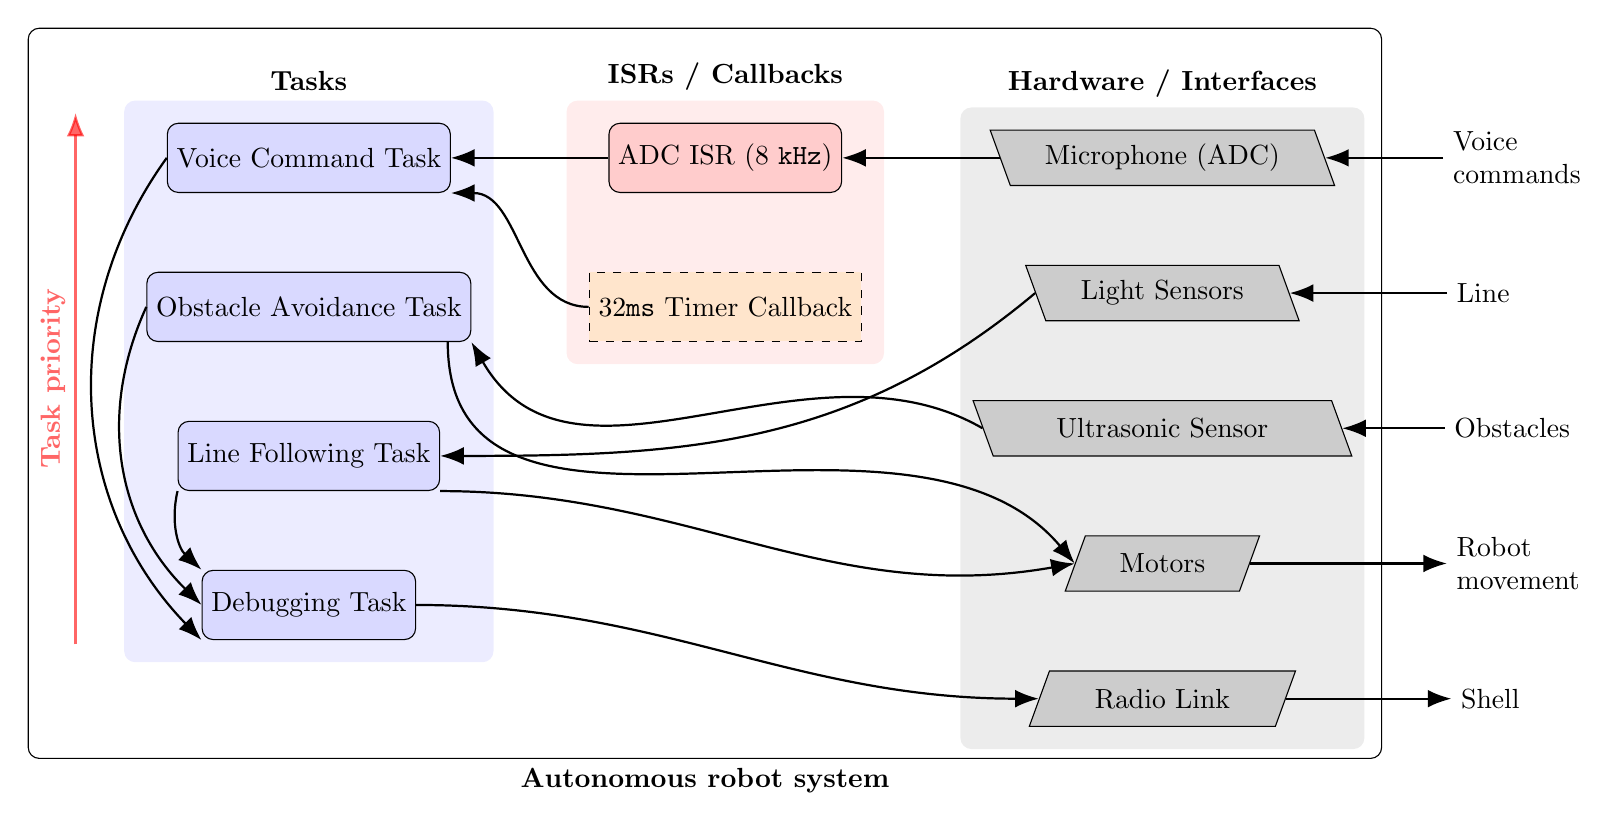
\begin{tikzpicture}[node distance=1cm and 2cm]

  % Hardware blocks
  \node (mic) [hw_in] {Microphone (ADC)};
  \node (light) [hw_in, below=of mic] {Light Sensors};
  \node (ultra) [hw_in, below=of light] {Ultrasonic Sensor};
  \node (motor) [hw_out, below=of ultra] {Motors};
  \node (radio) [hw_out, below=of motor] {Radio Link};

  % ISR and callbacks
  \node (adc_isr) [isr, left=of mic] {ADC ISR (8 \texttt{kHz})};
  \node (timer_cb) [callback, below=of adc_isr, yshift=0cm] {32\texttt{ms} Timer Callback};

  % Tasks
  \node (audio_task) [task, left=of adc_isr] {Voice Command Task};
  \node (obs_task) [task, below=of audio_task] {Obstacle Avoidance Task};
  \node (line_task) [task, below=of obs_task] {Line Following Task};
  \node (radio_task) [task, below=of line_task] {Debugging Task};

  % Groups
  \begin{scope}[on background layer]
    \node[group, draw=black,
    fit=(mic)(light)(ultra)(radio)(motor)(adc_isr)(timer_cb)(audio_task)(obs_task)(line_task)(radio_task),
    label=below:{\bf Autonomous robot system},
    xshift=-0.5cm, yshift=0.4cm,
    inner xsep=1cm, inner ysep=0.8cm] {};

    \node[group, fill=black, opacity=0.075,
    fit=(mic)(light)(ultra)(radio)(motor),
    label=above:{\bf Hardware / Interfaces}] {};
    \node[group, fill=red, opacity=0.075,
    fit=(adc_isr)(timer_cb),
    label=above:{\bf ISRs / Callbacks}] {};
    \node[group, fill=blue, opacity=0.075,
    fit=(audio_task)(line_task)(obs_task)(radio_task),
    label=above:{\bf Tasks}] {};
  \end{scope}

  % Arrows
  \draw [arrow] (mic.west) to (adc_isr.east);
  \draw [arrow] (light.west) to[out=220, in=0] (line_task.east);
  \draw [arrow] (ultra.west) to[out=150, in=300] (obs_task.south east);

  \draw [arrow] (obs_task.south east) ++(-0.3,0) to[out=270, in=130] (motor.west);
  \draw [arrow] (line_task.south east) to[out=0, in=190] (motor.west);
  \draw [arrow] (adc_isr.west) to (audio_task.east);
  \draw [arrow] (timer_cb.west) to[out=180, in=0] (audio_task.south east);
  \draw [arrow] (radio_task.east) to[out=0, in=180] (radio.west);

  \draw [arrow] (audio_task.west) to[bend right=40] (radio_task.south west);
  \draw [arrow] (obs_task.west) to[bend right=35] (radio_task.west);
  \draw [arrow] (line_task.south west) to[bend right=30] (radio_task.north west);

  \draw[arrow, red, opacity=0.6]
  (radio_task.west) ++ (-1.6,-0.5) -- ++(0,6.75)
  node[midway, above, rotate=90] {\bf Task priority};

  % System interations
  \node (mic_input) [right=of mic, xshift=-0.5cm, align=left] {Voice \\ commands};
  \node (light_input) [right=of light] {Line};
  \node (ultra_input) [right=of ultra, xshift=-0.7cm] {Obstacles};
  \node (motor_input) [right=of motor, xshift=0.5cm, align=left] {Robot \\ movement};
  \node (radio_input) [right=of radio, xshift=0.1cm] {Shell};

  \draw [arrow] (mic_input.west) to (mic.east);
  \draw [arrow] (light_input.west) to (light.east);
  \draw [arrow] (ultra_input.west) to (ultra.east);
  \draw [arrow] (motor.east) to (motor_input.west);
  \draw [arrow] (radio.east) to (radio_input.west);

\end{tikzpicture}

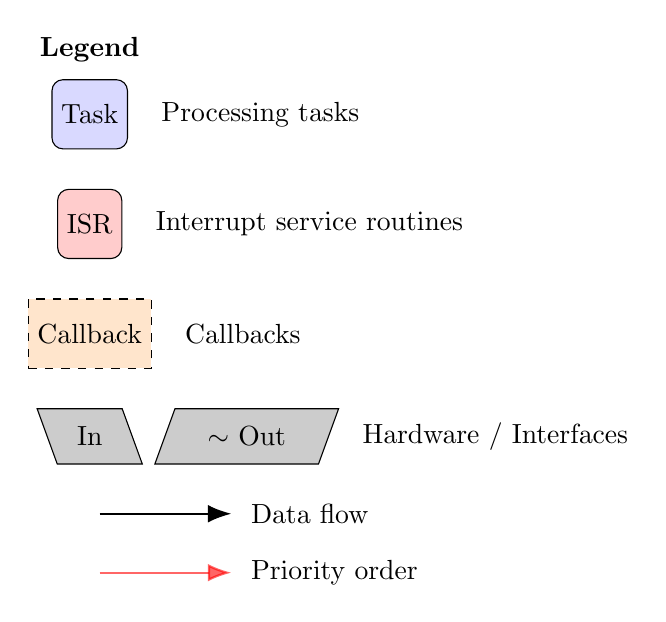
\begin{tikzpicture}[node distance=0.1cm and 0.3cm]

  \node (legend) {\bf Legend};

  \node[task, below=of legend] (task) {Task};
  \node[right=of task] {Processing tasks};

  \node[isr, below=0.5cm of task] (isr) {ISR};
  \node[right=of isr] {Interrupt service routines};

  \node[callback, below=0.5cm of isr] (cb) {Callback};
  \node[right=of cb] {Callbacks};

  \node[hw_in, below=0.5cm of cb] (hw_in) {In};
  \node[hw_out, right=0.4cm of hw_in] (hw_out) {\( \sim \) Out};
  \node[right=of hw_out] {Hardware / Interfaces};

  \node[draw=none, below=0.5cm of hw_in] (arr_label) {};
  \draw[arrow] (arr_label) -- ++(1.8,0);
  \node[right=1.8cm of arr_label] {Data flow};

  \node[draw=none, below=0.5cm of arr_label] (prio_label) {};
  \draw[arrow, red, opacity=0.6] (prio_label) -- ++(1.8,0);
  \node[right=1.8cm of prio_label] {Priority order};

\end{tikzpicture}

\end{document}
